\subsection{Reputation (aggregated trust matrix)}
In HOPR, we assume the majority of nodes are honest and act properly. Nevertheless, there might be nodes who actively try to attract the network by:
\begin{itemize}
    \item Dropping packets or acknowledgements
    \item Sending falsy packets, tickets or acknowledgements
\end{itemize}
Since nodes need to monitor the network to select paths, they need to filter nodes that behave inappropriately. 
In order to do so, we use a reputation system which gives a score to each node that acts as a relayer. 
\\The node’s reputation either increases or decreases its probability of being chosen depending on its behavior.

\subsubsection{Transitive trust evaluation }  
The reputation can be defined as: “a peer’s belief in another peer’s capabilities, honesty and reliability based on the other peers recommendations.”
Trust is represented by a triplet (trust, distrust, uncertainty) where:
\begin{itemize}
    \item Trust: $td^t(d,e,x,k)=\frac{n}{m}$ where $m$ is the number of all experiences and $n$ are the positive ones
    \item Distrust: $tdd^t(d,e,x,k)=\frac{l}{m}$ where $l$ stands for the number of the trustor’s negative experience.
    \item Uncertainty = 1 - trust - distrust.
\end{itemize}

\subsubsection*{Sequential propagation}
Assume that the trustor $a$ trusts $b$’s believes with: 
$tr(a,b,x,k)=<(td^b,dtd^b)>$ and $b$ trusts $c$’s performance with: 
$tr(b,c,x,k)=<(td^p,dtd^p)>$, then the trust relationship from $a$ to $c$ can be derived as follows:
$$td^p(a,c,x,k)=td^b(a,b,x,k).td^p(b,c,x,k)+ dtd^b(a,b,x,k).dtd^b(b,c,x,k)$$
$$dtd^p(a,c,x,k)=dtd^b(a,b,x,k).td^p(b,c,x,k) + td^b(a,b,x,k).dtd^b(b,c,x,k)$$

\subsubsection*{Parallel propagation}
Assume that entity $a$ trusts (directly or indirectly) entities $b_1,........,b_n$ with a certain degree and that entities $b_1,........,b_n$ trust the entity $c$ with some degree, the aggregation of trust from $a$ to the entity $c$ is:
$$td_g(a,c)=1-\prod_{i=1..n}(1-td_i) \quad and \quad dtd_g(a,c)=\prod_{i=1..n}dtd_i$$
where $<td_i,dtd_i>$ is the sequential aggregation of trust degree between $a$ and $c$ throughout the path $a->b_i->c$.

\subsubsection{Evaluation of trust}
\paragraph{Step1: Partial Trust}
Nodes can create small groups of neighbors, inside each group, nodes challenge one another using different testing techniques to figure out which members of the group are honest or malicious. 
These challenges will allow every node to construct trust knowledge about its neighbors. 
\begin{figure}
    \centering
    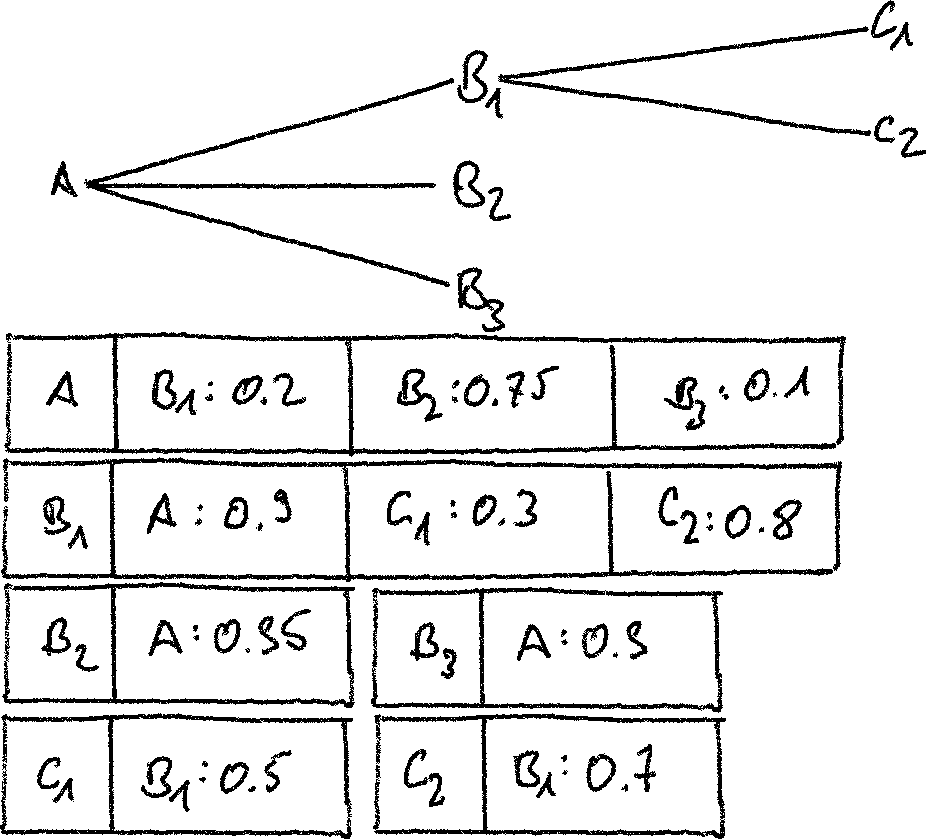
\includegraphics[width=7cm,height=7cm,keepaspectratio]{../whitepaper/images/reputation.png}
    \caption{Evaluation of trust}
    \label{fig:Evaluation of trust}
\end{figure}

\paragraph{Step2: Global Trust}
In order to compute the global trust, all nodes must collaborate and share their collective partial trust values with everyone on the network. 
\\We create a ”matrix of trust” that contains the trust degrees given by each entity of the network towards its neighbors. 
The final trust given to a by the network is the average of all inputs given by the other nodes in the network.





